\documentclass[11p, titlepage, oneside, a4paper]{article}
% Packages
\usepackage{amsmath}
\usepackage{graphicx}
\usepackage{hyperref}
\usepackage[english,swedish]{babel}
\usepackage[
    backend=biber,
    style=authoryear-ibid,
    sorting=ynt
]{biblatex}
\usepackage[utf8]{inputenc}
\usepackage[T1]{fontenc}
%Källor
\addbibresource{mall.bib}
\graphicspath{ {./images/} }

% Ändra de rader som behöver ändras
\def\inst{Teknikprogrammet}
\def\typeofdoc{Laborationsrapport}
\def\course{Fysik 1 150p}
\def\pretitle{Laboration 1}
\def\title{Rörelse: Hastighet och acceleration}
\def\name{Oscar Tafvelin}
\def\username{oscar.tafvelin}
\def\email{\username{}@ga.ntig.se}
\def\graders{Magnus Silverdal}

\begin{document}

\begin{titlepage}
		\thispagestyle{empty}
		\begin{large}
			\begin{tabular}{@{}p{\textwidth}@{}}
				\textbf{NTI gymnasiet \hfill \today} \\
				\textbf{\inst} \\
				\textbf{\typeofdoc} \\
			\end{tabular}
		\end{large}
		\vspace{10mm}
		\begin{center}
			\LARGE{\pretitle} \\
			\huge{\textbf{\course}}\\
			\vspace{10mm}
			\LARGE{\title} \\
			\vspace{15mm}
			\begin{large}
				\begin{tabular}{ll}
					\textbf{Namn} & \name \\
					\textbf{E-mail} & \texttt{\email} \\
				\end{tabular}
			\end{large}
			\vfill
            
\includegraphics[width=0.5\textwidth]{images/NTI Gymnasiet_Symbol_print_svart.png}
			\vfill
            \large{\textbf{Handledare}}\\
			\mbox{\large{\graders}}
		\end{center}
	\end{titlepage}

    \begin{otherlanguage}{english}
	\begin{abstract}
        We were given the task to calculate the speed of an object rolling down an incline. To do this we used a real life model that we rolled down a small incline and then used a program called "Tracker" on physlets.org to calculate the distance traveled and the amount of time it took to travel that distance. The program measured the distance and time and printed out measurements for both time and distance.
    \end{abstract}
    \end{otherlanguage}
    % Om arbetet är långt har det en innehållsförteckning, annars kan den utelämnas
	\pagenumbering{roman}
	\tableofcontents
	
	% och lägger in en sidbrytning
	\newpage

	\pagenumbering{arabic}
	
	% i Sverige har vi normalt inget indrag vid nytt stycke
	\setlength{\parindent}{0pt}
	% men däremot lite mellanrum
	\setlength{\parskip}{10pt}
	
	\section{Syfte och frågeställning}
		Syftet med laborationen är att analysera rörelse för en vagn som rullar längs en bana och beräkna hastighet och acceleration under rörelsen.

	\section{Bakgrund och teori}
        Med utgångspunkt från en film av förloppet kan mjukvara för motion tracking utnyttjas för att få fram vagnens position vid olika tidpunkter. Denna information används sedan tillsammans med definitionerna av medelhastighet $v_m = \frac{\Delta s}{\Delta t}$ och medelacceleration $a_m = \frac{\Delta v}{\Delta t}$ för att beräkna ett approximativt värde för hastigheten och accelerationen som funktion av tiden. Med ett tillräckligt kort tidssteg så blir medelvärdet ungefär lika med momentanvärdet och i filmen är tidssteget som störst $\frac{1}{25}$ sekund.  \parencite{impuls}
	

	\section{Metod och materiel}
        \begin{enumerate}
            \item Vagn
            \item Lutande plan med ställning
            \item Linjal
            \item Mobilkamera
        \end{enumerate}
        
        Det lutande planet monteras på ställningen så att den ena änden är 1 dm över bordet, se figur \ref{fig:lutandeplan}. Linjalen placeras längs planet så att det finns en längdskala  i filmen. Kameran placeras vid sidan av uppställningen på ett avstånd så att hela rörelsen ryms i filmen utan att kameran behöver flyttas. Vagnen rullas nedför planet samtidigt som kameran filmar rörelsen. Försöket placeras så att ljusförhållanden och bakgrund ger en så tydlig och skarp film som möjligt.
        
        \begin{figure}[!h]
            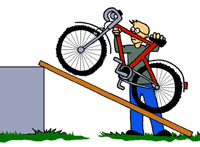
\includegraphics[width=0.8\textwidth]{images/lutandePlan.jpg}
            \caption{En blid hade varit superbra här}
            \label{fig:lutandeplan}
        \end{figure}
        
        Filmen analyserades sedan med mjukvaran Tracker för att få fram en tabell med positionen som funktion av tiden.
    \newpage
	\section{Analys och beräkning}
        Datat från analysen av filmen visas i tabell \ref{table:result}
    
        
        \begin{table}
            \begin{center}
            \begin{tabular}{ |c|c| } 
                \hline
                Position (m) & Tid (s)  \\ 
                \hline
                0 & 0  \\ 
                0.1 & 0.02 \\
                \vdots & \vdots \\
                \hline
            \end{tabular}
                \caption{Mätvärden}
                \label{table:result}
            \end{center}
        \end{table}            
        

    Datat importeras i Excel och hastigheten beräknas med hjälp av formeln
    \begin{equation}
        v_m = \frac{\Delta s}{\Delta t}
    \end{equation}
    
    \section{Slutsats och resultat} 
        Resultatet av beräkningarna illustreras i graferna 2 och 3
    \section{Diskussion} 
    Resultatet som vi fick fram med experimentet kanske inte är perfekt. Vi exkluderade vissa mätvärden på grund av att programmet strulade lite grann när mätningarna genomfördes. Till exempel så räknade den med ett par minusvärden i början som vi blev tvungna att ta bort. På grund av detta kanske man kan ifrågasätta hur exakta våra mätvärden faktiskt är.

    
    \printbibliography

\end{document}

